\section{Preliminary Results}\label{sec:results}
All runs below use the processed inputs the scMINER authors released, so differences from the paper do not come from our preprocessing. Our own implementation of the MICA distance matches the authors' code to $10^{-6}$ on about 10,000 random cell pairs, and we use it for the neighbor search.

\begin{table}[t]
\centering
\caption{MICA on the authors' released inputs, all genes, scored by the paper's rule (the true number of types is given and the labels pick the setting). ARI.}
\label{tab:repro}
\footnotesize
\setlength{\tabcolsep}{3.5pt}
\begin{tabular}{lrcccc}
\toprule
 & & \multicolumn{2}{c}{MICA} & Scanpy & Leiden \\
\cmidrule(lr){3-4}
Dataset & Cells & paper & ours & paper & ours \\
\midrule
Yan & 124 & 0.939 & 0.939 & 0.839 & 0.789 \\
Goolam & 124 & 0.544 & 0.544 & 0.572 & 0.308 \\
Buettner & 182 & 0.934 & 0.934 & 0.277 & 0.268 \\
Pollen & 249 & 0.942 & 0.951 & 0.874 & 0.858 \\
Chung & 317 & 0.655 & 0.655 & 0.170 & 0.319 \\
Usoskin & 622 & 0.847 & 0.835 & 0.860 & 0.598 \\
Kolodziejczyk & 704 & 1.000 & 0.727$^\ast$ & 0.996 & 0.564 \\
Klein & 2,717 & 0.980 & 0.980 & 0.820 & 0.977 \\
Zeisel & 2,903 & 0.744 & 0.764$^\dagger$ & 0.630 & 0.839 \\
PBMC14K & 13,605 & 0.853 & 0.854$^\dagger$ & 0.754 & 0.878 \\
\bottomrule
\end{tabular}
\\[2pt]
\parbox{\columnwidth}{\scriptsize $^\dagger$Graph mode, median of six runs (PBMC14K 0.850 to 0.857, Zeisel 0.755 to 0.781). Other rows use MICA's small-data mode with the final $k$-means given 100 restarts. $^\ast$Not reproduced from the released files (Sec.~\ref{sec:results}). The paper's Scanpy used 2,000 variable genes. Our Leiden uses all genes, the same input MICA gets, median of three seeds.}
\end{table}


\subsection{Reproduction}
MICA comes within 0.05 of the published ARI on 9 of 10 datasets (Table~\ref{tab:repro}), and to three decimals on six of them. Two details mattered. In small-data mode MICA ends with a single $k$-means call, and with the 10 restarts of its default setup it often stops at a worse local optimum (Yan scores 0.77 instead of 0.939). The published scores match the best fit, which took 100 restarts. Zeisel was run in graph mode by the authors' own scripts, and our six graph-mode runs give 0.755 to 0.781 against the published 0.744. Kolodziejczyk does not reproduce. MICA scores 0.727 on the released input, the same as the authors' own notebook, and their 1.0 seems to come from an input file that is not in the release.

The table also exposes a confound in the paper's comparison. Scanpy was run on 2,000 variable genes while MICA got all genes. Given all genes, the same input MICA sees, Leiden reaches 0.878 on PBMC14K and 0.839 on Zeisel, ahead of MICA on both.

\begin{table}[t]
\centering
\caption{Choosing the final clustering without and with the labels, on the authors' PBMC14K and Zeisel inputs with all genes (7 types in each). ARI as median [min, max] over six MICA graph-mode runs or three Leiden seeds, and $k$, the number of clusters chosen. In the top block the labels are used only to score.}
\label{tab:selection}
\scriptsize
\setlength{\tabcolsep}{2.4pt}
\begin{tabular}{llcccc}
\toprule
 & & \multicolumn{2}{c}{PBMC14K} & \multicolumn{2}{c}{Zeisel} \\
\cmidrule(lr){3-4}\cmidrule(lr){5-6}
Rule & Method & ARI & $k$ & ARI & $k$ \\
\midrule
\multicolumn{6}{l}{\textit{No labels}} \\
Default & MICA & 0.844 [0.84, 0.85] & 7 & 0.608 [0.54, 0.72] & 9 to 11 \\
 & Leiden & 0.866 [0.85, 0.87] & 8 & 0.378 [0.37, 0.38] & 21 \\
Silhouette & MICA & 0.624 [0.62, 0.83] & 5 or 7 & 0.659 [0.63, 0.74] & 9 \\
 & Leiden & 0.397 & 4 & 0.370 [0.36, 0.37] & 2 \\
\midrule
\multicolumn{6}{l}{\textit{Labels pick the setting}} \\
Paper's rule & MICA & 0.854 [0.85, 0.86] & 7 & 0.764 [0.76, 0.78] & 7 \\
 & Leiden & 0.878 & 7 & 0.839 & 7 \\
\bottomrule
\end{tabular}
\end{table}


\subsection{Choosing the clustering without labels}
Table~\ref{tab:selection} answers the main question on the two anchor datasets, and AMI gives the same ordering in every row. When the labels pick the setting, Leiden is ahead on both. Without labels the picture changes in three ways.

First, Leiden falls much further than MICA on Zeisel. At its default it splits 7 types into 21 clusters (ARI 0.378), and the silhouette rule merges everything into 2 (0.370). MICA lands at 9 to 11 clusters under either rule (0.608 and 0.659). Against their label-chosen scores, Leiden loses 0.46 to 0.47 ARI and MICA loses 0.11 to 0.16.

Second, on PBMC14K the defaults are close (MICA 0.844, Leiden 0.866). The silhouette rule hurts both, but Leiden more, because it merges the data into 4 clusters.

Third, label-free MICA varies from run to run. On PBMC14K its silhouette pick is 5 clusters in four of six runs and 7 in the other two, which moves ARI from 0.62 to 0.83. Leiden barely changes across seeds. The paper's protocol hides both effects: how far each method falls when it must choose for itself, and how much a single run can mislead.

Over all ten datasets and four gene settings, silhouette-chosen ARI averages 0.572 for MICA and 0.542 for Leiden. That small lead changes sign when we change the range of $k$ or the embedding used for the silhouette, so we do not treat it as an answer yet. This is why the plan in Sec.~\ref{sec:plan} adds stronger label-free rules.

\begin{figure}[t]
\centering
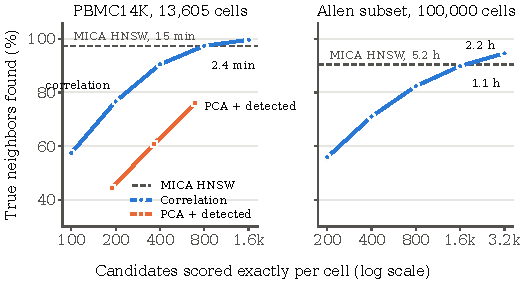
\includegraphics[width=\columnwidth]{figures/a2_neighbor_recall.pdf}
\caption{Share of each cell's 79 exact mutual information neighbors that a fast search finds, measured by brute force on 500 random cells. Candidates are scored with the exact MICA distance. Times are for building the graph for all cells with 8 CPU workers. The dashed line is MICA's own HNSW search.}
\label{fig:neighbors}
\end{figure}

\subsection{Neighbor search on subsets}
MICA's graph mode needs each cell's 80 nearest neighbors (the cell itself included), and its HNSW search for them is its slowest step. The feedback asked whether rescoring candidate pairs exactly can still miss important neighbors. So we found the exact neighbors of 500 random cells by brute force and measured the share each method recovers (Fig.~\ref{fig:neighbors}).

On PBMC14K, candidates from 50 principal components miss many neighbors even when merged with cells that share detected genes, finding 76\% with about 700 candidates per cell. Correlation over all genes, computed as one matrix product, does much better. With 800 candidates it finds 97.4\%, the same as MICA's HNSW (97.3\%), and the graph for all cells took 2.4 minutes against 15. We then fed both graphs to MICA's own later steps (node2vec and Louvain). Our graph gave ARI 0.853 in two runs, and MICA's graph gave 0.852 twice.

On 100,000 Allen cells brute force would take about 43 hours, so the subset sets the cost. HNSW finds 90.3\% of neighbors in 5.2 hours. Correlation finds 89.8\% with 1,600 candidates in 1.1 hours, and 94.6\% with 3,200 in 2.2 hours. Through MICA's later steps our 3,200 graph scores ARI 0.602 and 0.627, against 0.617 and 0.641 on MICA's graph (0.652 in MICA's own run), and its AMI is about 0.01 lower in every run. The candidates needed grow with the data (800 at 13,605 cells, 1,600 at 100,000), so the full 2.3 million cells would need a GPU version or a sketch.

Missed neighbors are not the whole story, though. The exact graph is crowded by hub cells. On PBMC14K the top 1\% of cells fill 23\% of all exact neighbor slots, and their links join cells of the same type only 42\% of the time, against 76\% for other links. On Klein, Leiden run directly on the exact graph scores 0.59, but up to 0.98 on approximate graphs that miss many true neighbors. So we judge a fast graph by the clustering it gives, not by recall alone.
